\documentclass[conference]{IEEEtran}
\ifCLASSINFOpdf
  % \usepackage[pdftex]{graphicx}
  % declare the path(s) where your graphic files are
  % \graphicspath{{../pdf/}{../jpeg/}}
  % and their extensions so you won't have to specify these with
  % every instance of \includegraphics
  % \DeclareGraphicsExtensions{.pdf,.jpeg,.png}
\else
  % or other class option (dvipsone, dvipdf, if not using dvips). graphicx
  % will default to the driver specified in the system graphics.cfg if no
  % driver is specified.
  % \usepackage[dvips]{graphicx}
  % declare the path(s) where your graphic files are
  % \graphicspath{{../eps/}}
  % and their extensions so you won't have to specify these with
  % every instance of \includegraphics
  % \DeclareGraphicsExtensions{.eps}
\fi

\usepackage{booktabs} % For formal tables
\usepackage{multirow}
\usepackage{algorithm}
\usepackage[noend]{algorithmic}
%\usepackage[noend]{algpseudocode}
\usepackage[pdftex]{graphicx}
\usepackage[T1,hyphens]{url}
\usepackage[dvipsnames]{xcolor}
%\usepackage[colorlinks,urlcolor=blue]{hyperref}
\usepackage[]{hyperref}
\usepackage{subfigure}
\usepackage{amsmath}
\usepackage{siunitx}
% \usepackage{align}
% \usepackage{authblk}

% \usepackage[style=alphabetic,maxnames=1,minnames=1,maxbibnames=99]{biblatex}

\graphicspath{{./figures/}}
%\algrenewcommand\textproc{}

%\algsetup{linenosize=\small}

% correct bad hyphenation here
\hyphenation{op-tical net-works semi-conduc-tor}

\begin{document}
%
% paper title
% Titles are generally capitalized except for words such as a, an, and, as,
% at, but, by, for, in, nor, of, on, or, the, to and up, which are usually
% not capitalized unless they are the first or last word of the title.
% Linebreaks \\ can be used within to get better formatting as desired.
% Do not put math or special symbols in the title.
\title{CNT-Cache: an Energy-Efficient Carbon Nanotube Cache with Adaptive Encoding}
% Ironing out the irregularity in BFS for efficient OpenCL implementation on Xeon-FPGA
%\author[1]{Dawen Xu}
%\author[1]{Kexin Chu}
%\author[2]{Cheng Liu}
%\author[2]{Ying Wang}
%\author[2]{Lei Zhang}
%\author[2]{Huawei Li}
%\affil[1]{School of Electronic Science \& Applied Physics Hefei University of Technology Anhui,China}
%\affil[2]{Institute of Computing Technology, Chinese Academy of Sciences,Beijing,China}
%\affil[]{\{xudawen@hfut,chukexin2017@mail.hfut\}.edu.cn, \{liucheng,wangying2009,zlei,lihuawei\}@ict.ac.cn}

% make the title area
\maketitle

% As a general rule, do not put math, special symbols or citations
% in the abstract
\begin{abstract}
    Carbon Nanotubu field-effect transistor (CNFET) that 
    promises both higher clock speed and energy efficiency 
    becomes an attractive alternative to the conventional 
    power-hungry CMOS cache. We observe that the CNFET-based cache 
    constructed with typical SRAM cells has distinct energy consumption 
    when reading/writing 0 and 1 from/to it. For instance, the energy consumption 
    of writing 1 to an SRAM cell is almost 10X higher than writing 0. 
    With this observation, we propose an energy-efficient cache design 
    called CNT-Cache to take advantage of this feature. It predicts the cache 
    line access pattern based on the latest cache line access history.  
    On top of the prediction, it decides the optimal cache line encoding 
    to match the cache operation preferences at runtime. According to 
    our experiments on a set of benchmark programs, the optimized CNFET-based 
    D-Cache reduces the dynamic power consumption by 22.2\% on average 
    compared to the baseline CNFET cache.
\end{abstract}

% For peer review papers, you can put extra information on the cover
% page as needed:
% \ifCLASSOPTIONpeerreview
% \begin{center} \bfseries EDICS Category: 3-BBND \end{center}
% \fi
%
% For peerreview papers, this IEEEtran command inserts a page break and
% creates the second title. It will be ignored for other modes.
\IEEEpeerreviewmaketitle

\section{Introduction} \label{sec:intro}
Inspired by the widespread adoption of neural networks in massive fields such as image classification, 
video surveillance, speech recognition, and robot vision, neural network accelerators 
\cite{Zhang2015_9,Qiu2016_10,deepburing_12,DiCecco_4,Zeng2018_18} 
are increasingly explored and deployed to improve the computing performance and energy efficiency.
Unlike generic applications, neural networks usually involve redundancy and are known to be 
fault tolerant\cite{Reagen2016}. By taking advantage of this feature, many neural network accelerator optimizations 
such as neural network pruning and low-precision quantization can be utilized to improve 
performance and energy efficiency notably with minor inference accuracy penalty\cite{Han2016DeepCC}. 

In line with these optimizations, we opt to relax the design constraints of 
the neural network accelerators, which provides a unique way to achieve notable 
improvements on performance or energy efficiency with small inference accuracy loss. 
For generic hardware design, strict design constraint is typically required to 
guarantee correct computing under even the most severe environments. On the contrast, 
neural network accelerators are more resilient and less sensitive to computing 
errors incurred by timing violations. Given relaxed design constraints, many 
aggressive hardware optimization techniques can be applied with computing errors. 
For instance, emerging techniques such as  near-threshold voltage regime\cite{RG2010NT} 
and subthreshold digital logic design\cite{BH2005,B2006} promise high energy efficiency 
but suffer instability\cite{Pu2010NT}. Conventional neural network accelerator 
can be pushed to operate at higher clock frequency with timing violations
\cite{overclock_3,Paceline_15}. At the fab level, design rules may also 
be aggressively pushed to reduce the expense. 

Motivated by the great advantages of relaxed design constraints,
we further explore the use of neural network resilience for more 
effective design trade-offs. When there are timing violations
and computing errors in the accelerator, the unmodified neural networks 
executed on the accelerators during inference is different 
from that computed on GPPs during the training, which may cause clear 
prediction accuracy loss. Instead of deploying the unmodified neural 
network models on the accelerators directly, we borrow the retraining 
idea from prior neural network quantization work \cite{Hwang2014_17,Matthieu2014_8} 
and have the deep neural network models to learn and tolerate the computing errors.  
Basically, we have the forward computing performed on the accelerator and 
then transfer the computing results to the host processor for 
backward propagation. With this approach, both application data and computing 
errors are learned and incorporated in the neural network models.  
Meanwhile, we define a set of standard interfaces to make it convenient 
to integrate general CNN accelerators into the retraining framework. 

In addition, we notice that some of the neural network layers are more sensitive to the 
computing errors and the sensitive layers dramatically limit the usefulness of the retraining. 
Thus, we schedule the most sensitive layer which is usually the last 
layer of the neural networks to host processors to reduce the negative influence 
of the computing errors. With both the retraining and sensitive layer protection, 
the neural networks become more resilient to the computing errors caused by 
the aggressive design options such as near-threshold logic or overclocking.
Compared to the original neural networks, the prediction accuracy of top-1 and top-5 
improves by 22.8\% and 9.89\% on average. The contributions of this work are 
summarized as follows.

\begin{itemize}
	\item We propose to improve the fault-tolerance of neural networks and make use of it to relax 
		the accelerator design constraints for higher performance or energy efficiency.

	\item We propose a neural network training framework to obtain resilient neural network models. 
		By integrating accelerator into conventional training, we have the computing errors 
		learned with the application data. By protecting the layer with most large errors, 
		we can further improve the resilience of the neural networks and pose more 
		opportunities to hardware optimizations.

	\item With comprehensive experiments, we show that the proposed training framework 
		could enhance the prediction accuracy of neural networks significantly 
		when the accelerators run with computing errors incurred by either 
		overclocking or lower voltage.
\end{itemize}
The paper is organized as follows. Section II analyzes the influence of 
the CNN accelerator computing errors on the neural network prediction accuracy. 
Section III presents the proposed training for neural networks executed on accelerators with computing errors.
Section IV demonstrate the use of the training on accelerators with overclocking and generic computing errors. 
Section V briefs the related work and Section VI draws the conclusion. 



\section{Related Work} \label{sec:relatedwork}
Despite of the performance and power advantages, the design 
productivity of developing FPGA applications remains low 
due to the lengthy compilation and complex application-specific 
customization. And it has become the major obstacle 
that hinders the wide adoption of FPGAs as commodity computing devices. 
The community from both the industry and academia have developed 
many different methods from diverse angles to tackle the problem. 
These methods can be roughly classified into three categories. 
The first category mainly focuses on improving the low-level 
implementation tools. A number of approaches such as making 
quality/runtime trade-offs \cite{mulpuri2001runtime}, parallel 
compilation \cite{moctar2014parallel, goeders2011deterministic, altera-pc, 
xilinx-pc} and using hard-macro techniques \cite{lavin2013improving, 
korf2011automatic} have been explored from this angle. The second 
category mainly centers the HLS design flow while the third one 
primarily relies on the overlay concept. They later two categories 
will be detailed in the following sections.

\subsection{High-Level Synthesis} 
With many years of continuous endeavor, a number of tools have emerged as 
mature solutions for HLS \cite{VivadoHLS, Legup, zhang2008autopilot}. They typically 
allow designers to express hardware designs using high-level  
description languages such as C, C++ etc. and also enable evaluation of different 
design choices using pragmas or directives. Indeed, they significantly improve 
the design productivity compared to the conventional hardware design flow using 
hardware description languages. However, when considering the overall design 
productivity of developing hybrid software-gateware applications, HLS is 
only addressing part of the problem, as the lengthy low-level compilation 
including synthesis, mapping, placing and routing remains a bottleneck for 
an application designer \cite{ROB2014, capalija2014tile}.

Customizing the generated hardware specifically to an user 
application is also time-consuming for designers and thus critical to the design 
productivity. A number of algorithms such as generic algorithms 
relied on local-search techniques \cite{schafer2009adaptive, 
sengupta1997genetic}, learning-based methods \cite{onlinecustomization, 
carrion2012machine}, divide and conquer algorithm \cite{DCcustomization} 
and a calibration free algorithm \cite{RCcustomization} etc. have been developed 
to perform the DSE on top of HLS tools. The algorithms can efficiently help automate the 
customization or DSE process. However, the algorithms must rely on HLS tools 
to estimate the implementation information such as implementation frequency, 
overhead or power for the corresponding customization. While the hardware generated 
can be irregular and may vary dramatically, thus the accuracy of the estimation 
especially on implementation frequency and power can be rather limited, which may
fail to optimize an HW/SW co-design problem.  

\subsection{Overlay Architectures}
Overlay architecture which is a virtual intermediate architecture overlaid on 
top of off-the-shelf FPGA is increasingly applied as a way to address the 
productivity challenge. 

Various overlays with diverse configuration granularities and flexibility 
ranging from virtual FPGAs \cite{Grant2011Malibu, ZUMA2012}, 
array-of-FUs \cite{mesh-FUs,ferreira2011fpga}, soft 
CGRA \cite{kissler2006dynamically, scgra-orig}, soft GPU \cite{Guppy2012GPU-Like}, 
vector processors\cite{Yiannacouras2009FPS, MXP2013} to 
configurable processors or multi-core processors \cite{unnikrishnan2009application, 
MARC2010, Yiannacouras2007Exploration, Capalija2009coarse-grain, OCTAVO2012, iDEA2012} 
have been developed over the years. SCGRA overlay provides unique 
advantages on compromising hardware implementation 
and performance for compute intensive nested loops as demonstrated 
by numerous ASIC CGRAs \cite{tessier2001reconfigurable, compton2002reconfigurable}.
Most importantly, it allows both rapid compilation by taking advantage of 
the overlays' tiling structure \cite{ROB2014} and efficient bitstream 
reuse within the design iterations of an application \cite{scgra-orig}, 
thus it is particularly promising for high productivity nested loop acceleration.

Despite of the promising potential, a complete automatic customization 
framework that enables application-specific optimization is still highly 
anticipated for the sake of design productivity and performance. 
The authors in \cite{colinheart} developed an SCGRA topology customization method 
using genetic algorithm and showed the potential benefits of the SCGRA 
overlay customization. However, the rest system design parameters such as 
on chip buffer size, loop unrolling factor etc. are not covered. 

Indeed, SCGRA overlays have many similarities in terms of array structure 
and scheduling algorithm with ASIC CGRAs. Nevertheless, ASIC CGRAs emphasize 
more on configuration capability and limited customization is allowed due 
to the overhead constraints \cite{zhou2014application, miniskar2014retargetable} 
while SCGRA overlays allow more intensive architectural customization 
because of the FPGA's inherent programmability. Moreover, hardware resources such as 
DSP blocks and RAM blocks available on FPGAs are discrete, which results in different 
design constraints for SCGRA overlay customization as well. 

By utilizing the SCGRA overlay as the backbone of the FPGA accelerator, 
a complete nested loop acceleration framework 
targeting CPU-FPGA system is developed. It supports intensive application-specific
customization including the overlay architectural customization, 
the compilation customization and communication interface customization 
for various design goals. When the customized design parameters are determined, 
corresponding hardware accelerator and software can be compiled to the target 
CPU-FPGA system rapidly eventually providing a push-button solution for a nested loop 
acceleration. 



\section{Energy Efficient CNFET-based Cache Design} \label{sec:warp}
The energy consumption of accessing '0' and '1' in CNFET-based SRAM cell 
differs dramatically. By taking advantage of the feature, we propose 
an adaptive run-time encoding approach and build an energy efficient 
CNFET-based cache named CNT-Cache. The architecture as well as the 
encoding approach will be detailed in this section.

\begin{figure}
    \center{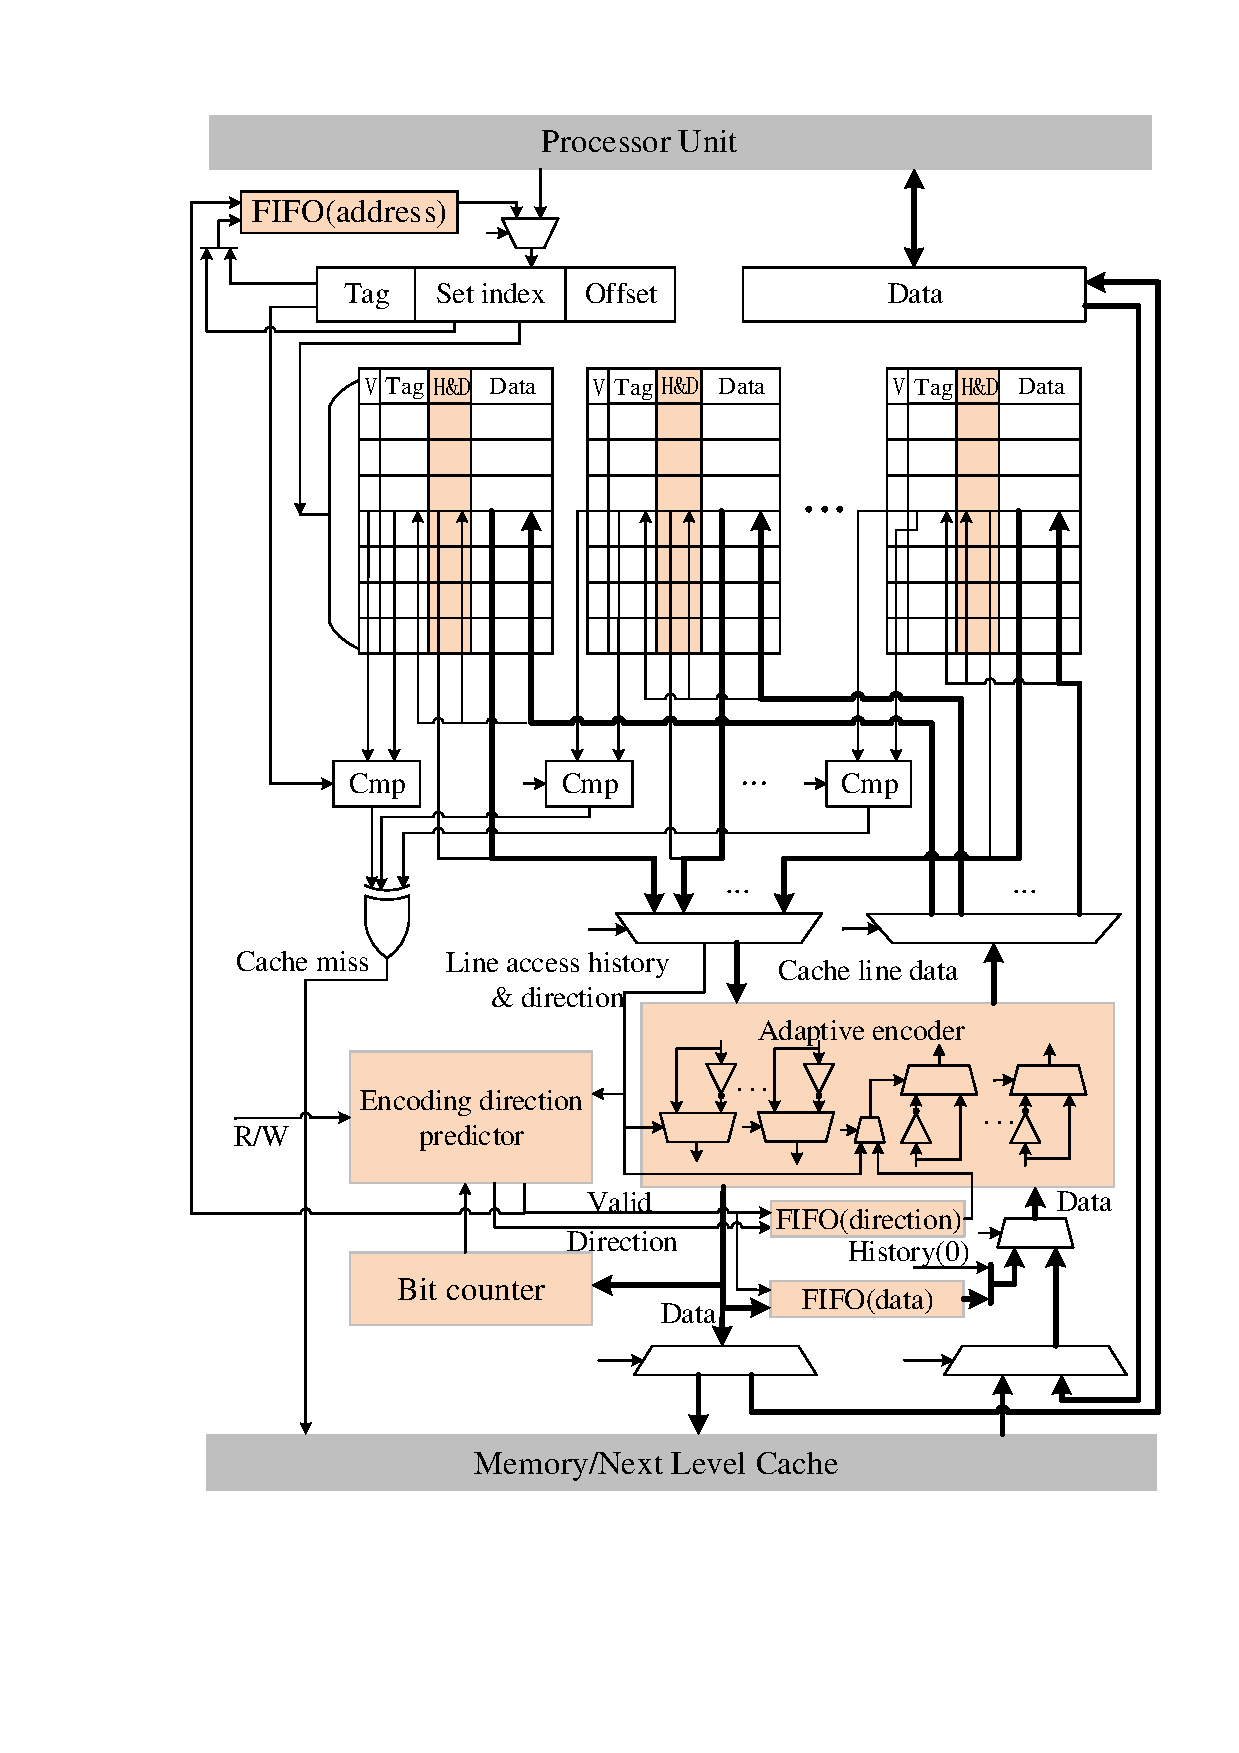
\includegraphics[width=0.88\linewidth]{cache_archi}}
    \caption{Architecture of CNT-Cache}
\label{fig:architecture}
\vspace{-1em}
\end{figure}

\subsection{CNT-Cache Overview}
Figure \ref{fig:architecture} illustrates the proposed CNT-Cache 
architecture with adaptive encoding support.
Compared to a typical cache architecture, it requires a few additional 
components as highlighted in orange. The most critical part is the 
adaptive encoding module. It can encode each cache line data with 
either more '1' bits or '0' bits depending on the cache line operation 
preferences. For example, suppose the original data has more '1' bits and 
the operation is more efficient in handling '0' according 
to Table \ref{tab:rw-analysis}. Then we can encode the 
data by inverting each bits and have an additional bit to record the encoding 
direction. Note that the operation can either be read or write. Meanwhile, 
the adaptive encoder is essentially a series of inverters
with 2-to-1 multiplexers and operates based on the encoding direction bit read from 
each cache line. The simple structure has negligible influence 
on the timing of the critical data path. 

Another key component is the encoding direction predictor. 
It determines the encoding pattern or preference of each cache line based on 
a window of historical accesses. With the access pattern (i.e. the number of read 
and the number of write in a window), it checks whether the current cache 
line data matches the cache line encoding direction.
If the current encoding does not fit the cache line data, we
change the encoding direction and update the cache line data accordingly.
To avoid affecting the cache write data path, a data FIFO is used to delay the update
until there is an idle time slot. Meanwhile, an index FIFO is also needed to 
decide the update cache line address synchronously. Also the cache line history 
will be reset. If there is no need to change the encoding,
we just update the cache access counter in history region in the cache line.
To enable encoding direction prediction of each cache line, we have each 
cache line access history stored along with the cache line data. Therefore, we need to 
widen the cache line to store the access history as well 
as the encoding direction. The added bits are marked as 'H\&D' (history and direction) in Figure \ref{fig:architecture}.

In general, the proposed CNT-Cache adjusts the cache line encoding 
based on the cache line data access pattern to minimize the overall 
cache access energy consumption. The encoding is in the cache 
operation data path, so it must be simple for efficient 
hardware implementation. The predictor determines the cache line 
encoding direction based on the access history in a window as 
well as the encoding switch overhead. It requires more computing 
but will not affect the critical data paths of the cache operations. 

\subsection{Cache line data encoder}
The cache line data encoder operates based on the encoding direction 
read from the corresponding cache line. When there are less 
preferred bits in the cache line data, typically we need to invert 
the whole cache line. Nevertheless,
this approach may fail to explore the continuous preferred bits 
in the data and convert them to bits that are inefficient for 
the cache operations. To address this problem, we adopt a fine-grained 
encoding approach to further reduce the inefficient bits in the data. 
Basically the input data is divided into multiple partitions and 
each partition is encoded independently to maximize the preferred bits.
In this case, % each partition needs one bit to record the encoding direction and 
we need to add more direction bits to each cache line.

To help illustrate the partitioned encoding, an example is presented in 
Figure \ref{fig:encode}. The raw data has much more '0' bits than '1' bits.
When the cache line is read intensive, %according to the encoding direction, 
the data needs to be inverted using the baseline encoding approach. 
In this case, the $(K-1)$th partition of the cache line data with more '1' bits 
are inverted though they are preferred for cache read. 
When the partitioned encoding approach is applied, the $(K-1)$th 
partition remains unchanged. Similar optimization opportunities can also be explored 
when the cache line is write intensive. Compared to the baseline encoding,
the partitioned encoding needs more direction bits.

\begin{figure}
    \center {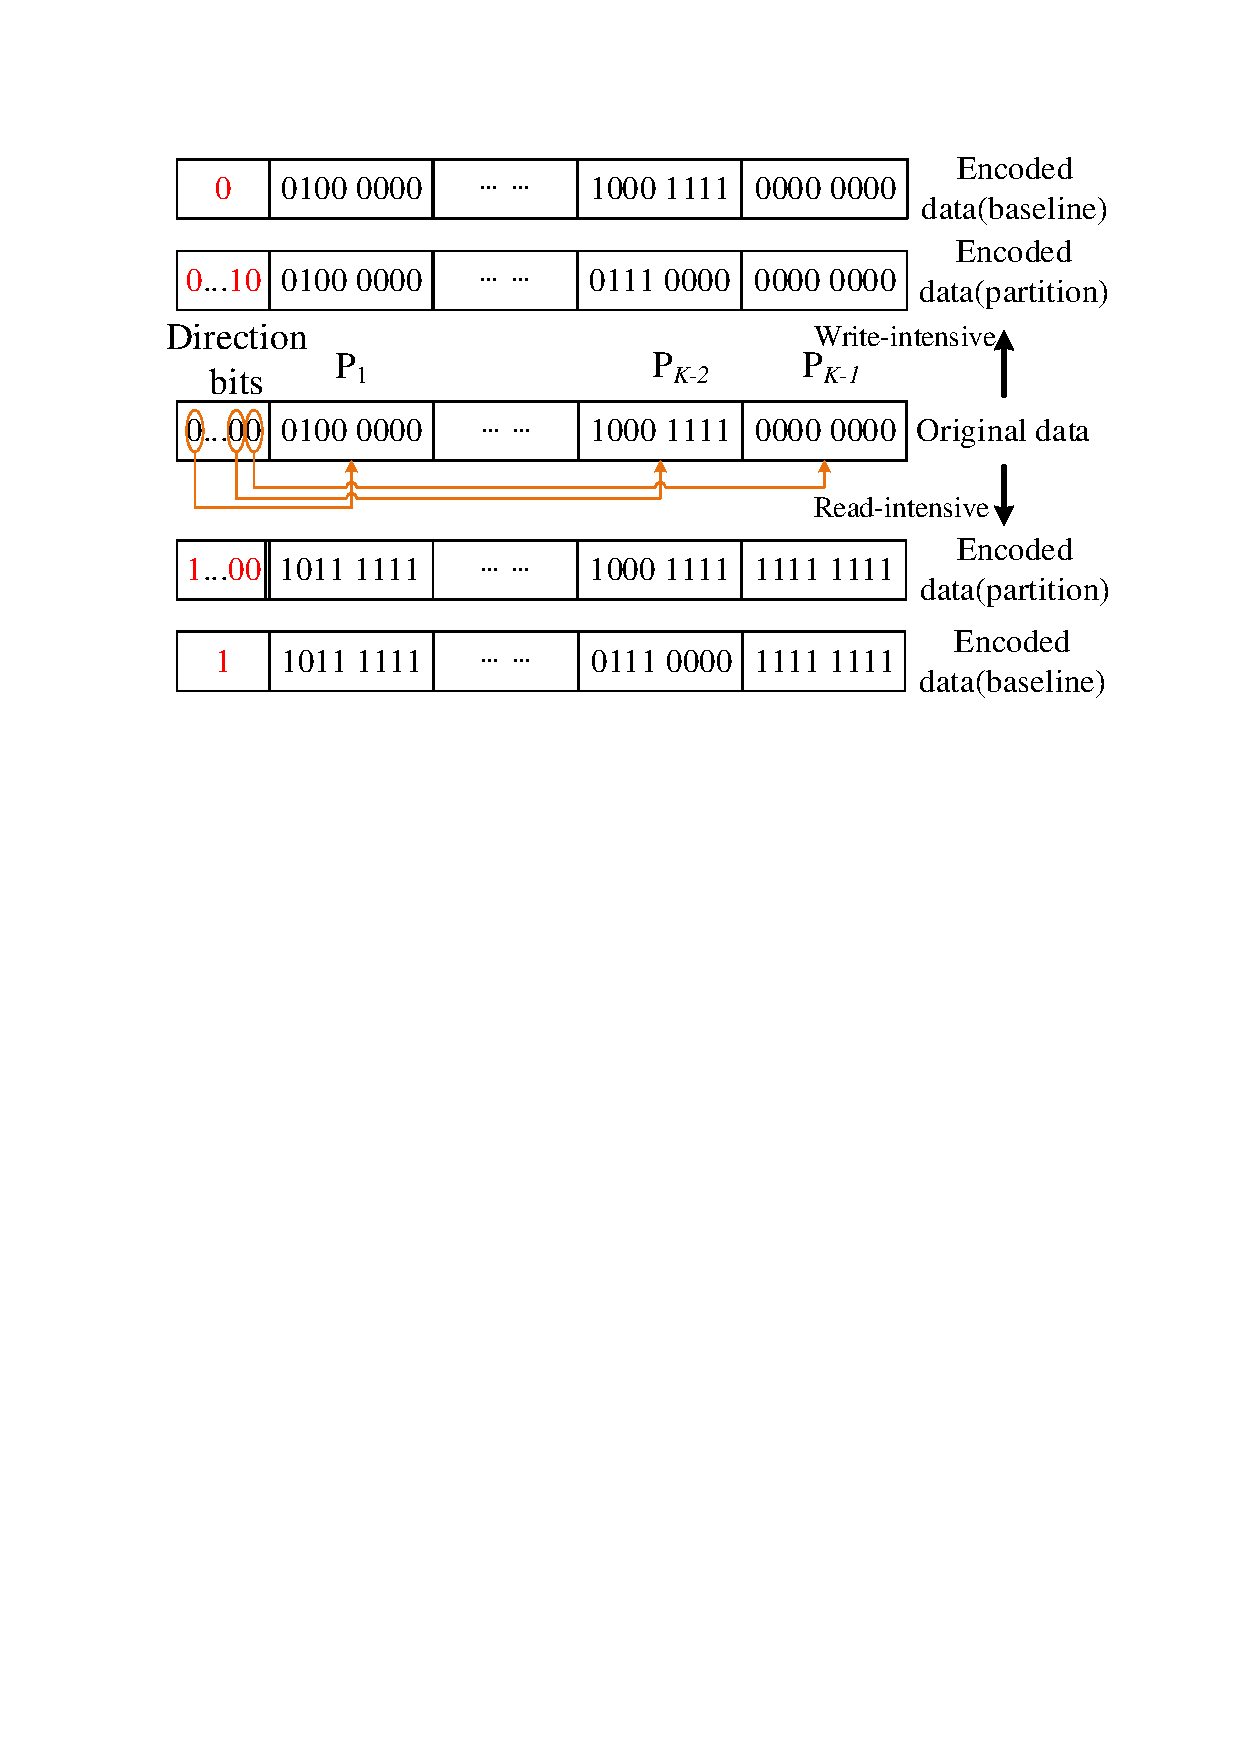
\includegraphics[width=0.85\linewidth]{encode}}
    \caption{An example of partitioned cache line encoding}
\label{fig:encode}
\vspace{-1em}
\end{figure}

The adaptive encoding module is essentially a series of inverters and 2 to 1 multiplexers
as described in Figure \ref{fig:architecture}.
When the partitioned encoding approach is utilized, the select signal of the multiplexers 
that are originally shared by the whole cache line data are now replaced with the partition 
direction bits instead. It has little influence on timing of the encoder module design. 

\subsection{Encoding direction predictor}
Encoding direction predictor determines the encoding of each cache line data.
It is of vital importance to the energy efficiency of the CNT-Cache.
While achieving optimal encoding for each cache access may cause frequent encoding 
direction switch and the switch overhead is non-trivial, thus the predictor 
performs prediction in the granularity of a window of accesses and decides if the encoding 
should be updated.

The proposed prediction strategy can be roughly divided into two steps as 
shown in Algorithm \ref{alg:prediction}. Firstly, we mainly analyze the operation 
preference of the cache line based on the access history. 
Basically, we keep a window $W$ of the latest accesses. 
$W$ also represents the prediction cycle. Within $W$, 
if the number of read is larger than a threshold $Th_{rd}$, 
it indicates that the cache line is read intensive. 
Otherwise, it is considered to be write intensive. 
The threshold is used to determine if it saves energy 
when we encode the stored data for reading. 
Suppose there are $x$ '0' bits and $y$ '1' bits on 
average in a window of accesses. Without loss of generality, assume $x<y$. 
The energy consumption using different encoding can be calculated with 
Equation \ref{eq:read_encoding_energy} and Equation \ref{eq:write_encoding_energy} 
respectively. Here $E_{rd0}$, $E_{rd1}$, $E_{wr0}$ and $E_{wr1}$ refer to 
the energy consumption of reading bit'0'/'1' and writing bit'0'/'1'. When $E_{rd\_enc}$ and $E_{wr\_enc}$ is equal, we can obtain $Th_{rd}$ using Equation \ref{eq:threshold}. 
Since $E_{rd0} - E_{rd1}$ is quite close to $E_{wr1} - E_{wr0}$ 
according to Table \ref{tab:rw-analysis}, $Th_{rd}$ is roughly half of $W$.

\begin{algorithm}
    \renewcommand{\algorithmicrequire}{\textbf{Input:}}
	\renewcommand{\algorithmicensure}{\textbf{Output:}}
    \caption{Encoding direction prediction algorithm} 
    \label{alg:prediction}
    \footnotesize
	\begin{algorithmic}[1] 
	    \REQUIRE Cache line access history including access 
	    number $A_{num}$, the number of write accesses $Wr_{num}$, and 
	    maximum access per prediction $W$, Cache line encoding direction $D$, 
	    Read intensive threshold $Th_{rd}$, Cache line data $Data$, 
	    Bit '1' number threshold array for encoding switch $Th_{bit1num}[W]$.
	    
	    \ENSURE Cache line access pattern ${Pattern}$, new encoding direction $D_{new}$ and 
	    new encoded data $Data_{new}$.
	    
	    \IF{($A_{num} = W$)}
	        \STATE
	        \STATE // Step 1: access pattern prediction
	        \IF{($Wr_{num} > Th_{rd}$)}
	            \STATE $Pattern \gets 1$ // write intensive
	        \ELSE
	            \STATE $Pattern \gets 0$ // read intensive
	        \ENDIF

            \STATE
            \STATE // Step 2: check if the cache line encoding will be changed.
	        \STATE $bit1num \gets getNumOfBit1(Data)$ // count '1' in $Data$
	        \IF {($Pattern = 1$)} %// write intensive
	            \IF{($bit1num > Th_{bit1num}[Wr_{num}]$)}
	                \STATE $D_{new} \gets \lnot D$
	                \STATE $Data_{new} \gets \lnot Data$
	            \ENDIF
	       \ELSE
	            \IF{($bit1num < Th_{bit1num}[Wr_{num}]$)}
	                \STATE $D_{new} \gets \lnot D$
	                \STATE $Data_{new} \gets \lnot Data$
	            \ENDIF
	       \ENDIF
	       
	       \STATE $A_{num} \gets 0$
	       \STATE $Wr_{num} \gets 0$
	       
	    \ELSE
	    	\STATE $Wr_{num} \gets Wr_{num} + 1$ when there is a cache write.
	        \STATE $A_{num} \gets A_{num} + 1$ when there is a cache access.
	    \ENDIF
	 
	%\EndProcedure
	\end{algorithmic}
\end{algorithm}

\footnotesize
\begin{equation}
    \label{eq:read_encoding_energy}
    \begin{split}
    E_{rd\_enc}=Th_{rd} \times (x \times E_{rd0} + y \times E_{rd1}) + \\ (W - Th_{rd}) \times (x \times E_{wr0} + y \times E_{wr1}) \\
    \end{split}
\end{equation}

\begin{equation}
    \label{eq:write_encoding_energy}
    \begin{split}
    E_{wr\_enc}=Th_{rd} \times (y \times E_{rd0} + x \times E_{rd1}) + \\ (W - Th_{rd}) \times (y \times E_{wr0} + x \times E_{wr1}) \\
    \end{split}
\end{equation}

\begin{equation}
\label{eq:threshold}
    \begin{split}
    % E_{rd\_enc} - E_{wr\_enc} = (y-x)(Th_{R/W} \times (E_{rd0} - E_{rd1}) + \\  (W-Th_{R/W}) \times (E_{wr0} - E_{wr1})) = 0 \\
    Th_{rd} = W \times \frac{1}{1 + \frac{E_{rd0} - E{rd1}}{E_{wr1}-E_{wr0}}}
    \end{split}
\end{equation}
\normalsize

As we predict the cache line read/write preferences using the two access 
counters i.e. $A_{num}$ and $Wr_{num}$, we need $2\times log{2}{W}$ 
bits to store them in each cache line. While it is usually expensive 
to add bits to the cache line, $W$ must be set properly to 
reduce the overhead of history bits.

In the second step, we mainly evaluate the current cache line data
and see if it fits the encoding and the access preferences in history, 
which is already determined in the first step. An intuitive approach 
is to calculate the energy efficiency of operating on the cache line 
data and compare with the cache access energy efficiency using a 
different encoding. If it consumes less energy, it means that the cache 
line data encoding is optimal. Otherwise, we need to reset the encoding 
and update the data stored in the cache line. 

The energy consumption of current cache line data access $E$ can be 
calculated using Equation \ref{eq:energy-efficiency}.
When a different encoding approach is used, the energy consumption 
becomes $\bar{E}$ as given in Equation \ref{eq:_energy-efficiency}.
Suppose $E_{encode}=N_{1} \times E_{wr0} + (L - N_{1}) \times E_{wr1}$ stands for the energy consumption of a cache 
line encoding switch which essentially updates the re-encoded data to cache.
When $E = \bar{E} + E_{encode}$, we can obtain the bit number ('1') threshold 
$Th_{bit1num}$ as presented in Equation \ref{eq:bit1num} 
where $E_{save} = (W-Wr_{num}) \times (E_{rd0}-E_{rd1}) - Wr_{num}\times(E_{wr1}-E_{wr0})$. 
Note that $bit1num$ represents the number of '1' bits in the data. 
It can be calculated using a bit counting function $getNumOfBit1()$ as described in 
Algorithm \ref{alg:prediction}. To make the representation short, 
we set $N_{1} = bit1num$. $L$ is the cache line length.

According to Equation \ref{eq:bit1num}, the threshold also depends on 
the cache line access history i.e. $Wr_{num}$ and it needs to be calculated at run-time.
Fortunately, we can obtain all the possible bit number threshold in advance 
and construct an array $Th_{bit1num}$ as presented in Algorithm \ref{alg:prediction}. 
The array can be implemented with a table that has $W$ entries. 
It returns the exact bit number threshold given $Wr_{num}$. In this case, the predictor 
can compare the number of bit '1' in the cache line with the threshold read from the 
table, and decides if it is necessary to inverse the encoding rapidly, which greatly 
simplifies the predictor design. 

\footnotesize
\begin{equation}
    \label{eq:energy-efficiency}
    \begin{split}
        %E=(W-Wr_{num}) \times (bit1num \times E_{rd1} + (L - bit1num) \times E_{rd0}) + \\
        %Wr_{num} \times (bit1num \times E_{wt1} + (L - bit1num) \times E_{wt0})
        E=(W-Wr_{num}) \times (N_{1} \times E_{rd1} + (L - N1) \times E_{rd0})\\
        + Wr_{num} \times (N_{1} \times E_{wr1} + (L - N1) \times E_{wr0})
    \end{split}
\end{equation}

\begin{equation}
    \label{eq:_energy-efficiency}
    \begin{split}
        %\bar{E}=(W-Wr_{num}) \times (bit1num \times E_{rd0} + (L - bit1num) \times E_{rd1}) + \\
        %Wr_{num} \times (bit1num \times E_{wt0} + (L - bit1num) \times E_{wt1})
        \bar{E}=(W-Wr_{num}) \times (N_{1} \times E_{rd0} + (L - N_{1}) \times E_{rd1}) \\ 
        + Wr_{num} \times (N_{1} \times E_{wr0} + (L - N_{1}) \times E_{wr1})
    \end{split}
\end{equation}

%\begin{equation}
%    \label{eq:energyencoding}
%    \begin{split}
%        E_{encode}=N_{1} \times E_{wr0} + (L - N_{1}) \times E_{wr1}
%    \end{split}
%\end{equation}

%\begin{equation}
%    \label{eq:save}
%        E_{save} = (W-Wr_{num}) \times (E_{rd0}-E_{rd1}) - Wr_{num}\times(E_{wr1}-E_{wr0})
%\end{equation}

\begin{equation}
    \label{eq:bit1num}
    \begin{split}
        N_{1} = \frac{L \times (E_{save} - E_{wr1})}{2\times E_{save} - (E_{wr1}-E_{wr0})}
    \end{split}
\end{equation}
\normalsize

%In addition, how to determine the data encoding pattern of the current cache block is the key to the effect of the above run-time encoding strategy. Because the misjudgment of each data encoding pattern will cause incorrect data encoding and sub-optimal performance.The sub-optimal performance can offset the overall optimization effect of the entire CNT-cache evenly. There are two things need to be considered when developing a effective judgment model: Firstly, the data encoding pattern of cache block should be determined by its previous access mode rather than recent access mode. Simply encoding data with its most recent access mode may result in frequent switching between different optimization patterns, which will cause energy waste. Secondly, the encoding phase should be removed from the critical path. For example, if every normal access to the cache needs to wait for the results of the prediction process, the delay it generates will significantly affect the performance of the cache.

%In general, the dynamic power consumption of cache in a period of time can be calculated by using the following formula:
%\begin{align}
%E = N_{allr} \times E_{avgr} + N_{allw} \times E_{avgw}
%\end{align}
%where, $N_{allr}$ and $N_{allw}$indicates the overall number of read- /write- accesses to the cache during run-time.$E_{avgr}$ and $E_{avg_w}$ represent the average read or write power consumption for a cache block. 
%However, in this article, not only how many cache blocks are read/written, but also the 0/1 number of stored data should be considered. So the above formula can be written as:
%\begin{align}
%E = \sum_{C=0}^N(E_{cache block})
%\end{align}
%\begin{align}
%E_{cache block} = E_{read} \times N_{read} + E_{write} \times N_{write}
%\end{align}
%\begin{align}
%E_{read} = N_{read0} \times E_{read0} + N_{read1} \times E_{read1}
%\end{align}
%\begin{align}
%E_{write} = N_{write0} \times E_{write0} + N_{write1} \times E_{write1}
%\end{align}
%Here $E_{cache block}$, $E_{read}$ and $E_{write}$ indicates the power consumption of one single cache block or one single read-/write to a cache block, $N_{read}$ and $N_{write}$ represents the number of read/write accesses to the cache block in a period if time. C and N are used to summarize the dynamic power consumption of all cache blocks during the period of time.

%Then, during the run-time of the system, we divide the run-time into small segments for each cache block(checkpoint), And record the number of accesses and write accesses to the current cache line during the checkpoint($AC$ indicates whether a checkpoint is completed and $WC$ indicates the number of write accesses). After that, the number of bit 0/1 in stored data will be recorded by Bit Counter, and the dynamic power consumption of each optimization direction will be calculated and compared. Finally, if the new direction performs better, the data encoding and write back processes will be started, updating the flag bits and real data while clearing other flag information. one thing to note here is that if the encoding direction changes, it will cause an additional writeback operation, so here a write operation is added when calculating the dynamic power consumption of the new direction, which means $E_{new} = E_{read} \times N_{read} + E_{write} \times (N_{write} + 1)$.

%Of course, it is unrealistic to calculated the above formula for each pattern prediction, because the formula above is too complicated. It is found that the TB(defined as the threshold for the number of Bits 1 when the mode changes) is related to the number of write accesses and k via calculation Within a limited number of accesses. Once these three values are determined, the TB is uniquely determined. Since the size of checkpoint and K are pre-set, only a small hash table(equal to the size of checkpoint) is needed to avoid all calculations.
	

%\subsubsection{Threshold}
%As mentioned above, firstly, the access power consumption can be reduced only by accurately predicting the access pattern of each cache block, because inaccurate access pattern prediction will only lead to higher waste of access energy. Secondly, the optimization type of the cache block should be determined by its previous access pattern, since simply encoding the data with the latest access mode may result in frequent switching between different optimization methods, which will cause additional energy wastage. In order to avoid inaccurate data encoding as much as possible, we introduce a threshold $\Delta$T to determine whether the optimization pattern of current cache block needs to be changed. The $\Delta$T indicates that the new encoding direction saves more than $\Delta$T of the original one during the checkpoint. In other words, the new pattern becomes the stable optimization pattern only when $E_{original} - E_{new} > \Delta T \times E_{original}$ is satisfied. In summary, the algorithm of the pattern predictor is shown in Algorithm.\ref{alg:prediction}. By default, we set checkpoint as 15 accesses operation to each cache block. And in order to save the maximum power overhead, we will explore the relationship between $\Delta$T and dynamic energy saving through a series of experiments. The results are shown in section\ref{sec:result}.

\section{Experiments}
In this section, we analyze the benefits of 
overclocking on a set of representative convolution neural networks.
and estimate the trade-offs of the strategies 
used to mitigate the overclocking incurred errors.

\subsection{Experiment setup}
We used PipeCNN as the baseline CNN accelerator and had it implemented on KCU1500 FPGA board.
Four representative neural networks including LeNet, AlexNet, VGG-16 and VGG-19 are used to 
benchmark the performance and energy efficiency of the CNN accelerator. The implementation clock
frequency of LeNet and AlexNet is 210 MHz while the clock frequency for VGG-16 and VGG-19 is 
190 MHz. Then we gradually overclock the implementation with 10 MHz step until the accelerator gets 
stuck or crashes frequently. For the 210 MHz implementation, the highest overclocking setup is 
260MHz. For the 190 MHz implementation, the highest overclocking setup is 240 MHz.
Finally, we evaluate the performance and energy efficiency of the accelerators using 
all the available overclocking configurations.

\subsection{Accuracy, performance and energy efficiency}
The prediction accuracy of the benchmark neural networks on the CNN accelerators with overclocking is 
presented in Fig \ref{fig:overclock-accuracy}. It can be found that the prediction accuracy 
regardless of top1 or top5 typically remains the same under moderate overclocking. However, when the clock 
continues to rise, it may reach to a tipping point where the prediction accuracy drops clearly. 
Fortunately, the prediction accuracy can be improved with just on-accelerator retraining.
When the clock further increases, the prediction accuracy drops dramatically. In spite of the retraining, 
the prediction accuracy is still not acceptable in practice. Part of the reasons can be that the 
number of timing violations increases rapidly with higher clock frequency. 
\begin{figure}
        \center
	\subfloat[LeNet]{
		\label{fig:lenet_accuracy}
		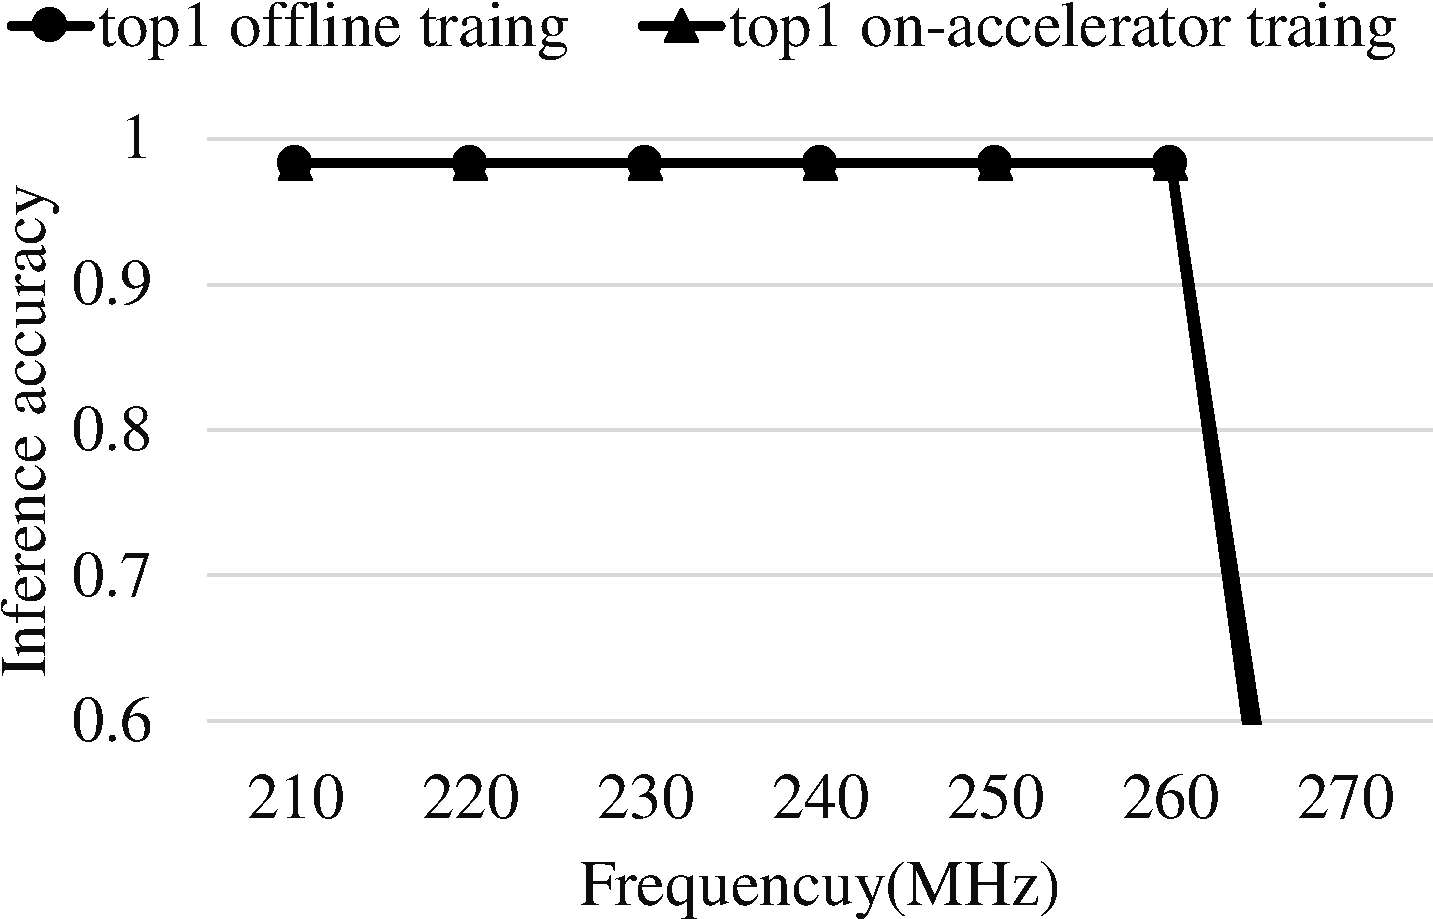
\includegraphics[width=0.65\linewidth]{accuracy_lenet}
	}
	\qquad
	\subfloat[AlexNet]{
                \label{fig:alexnet_accuracy}
                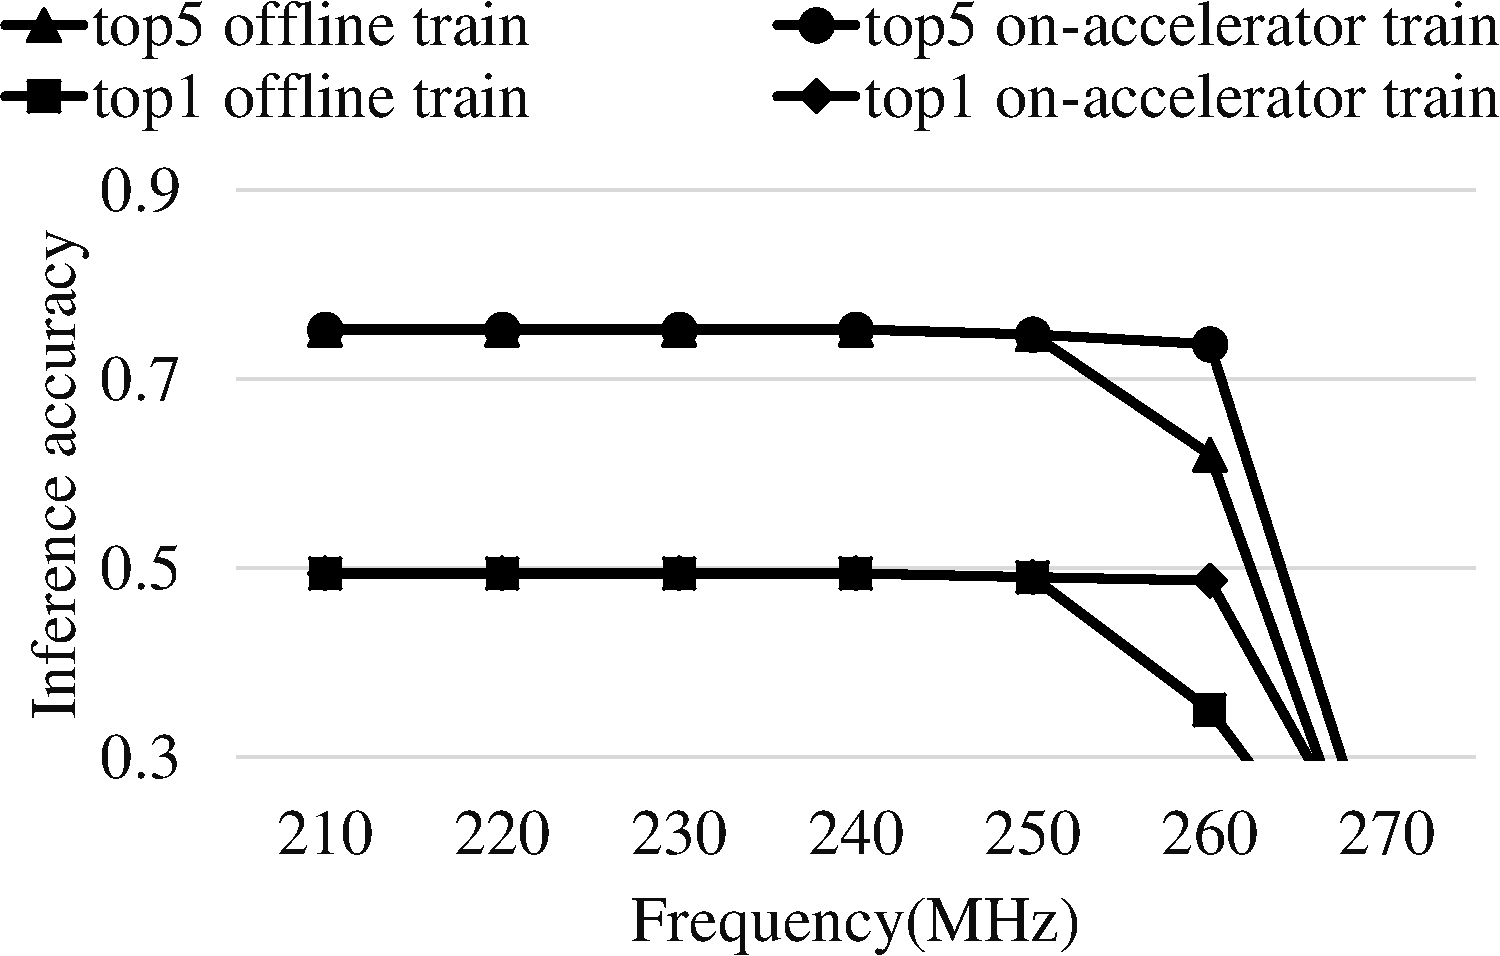
\includegraphics[width=0.65\linewidth]{accuracy_alexnet}
        }
	\qquad
	\subfloat[VGG-16]{
                \label{fig:vgg16_accuracy}
                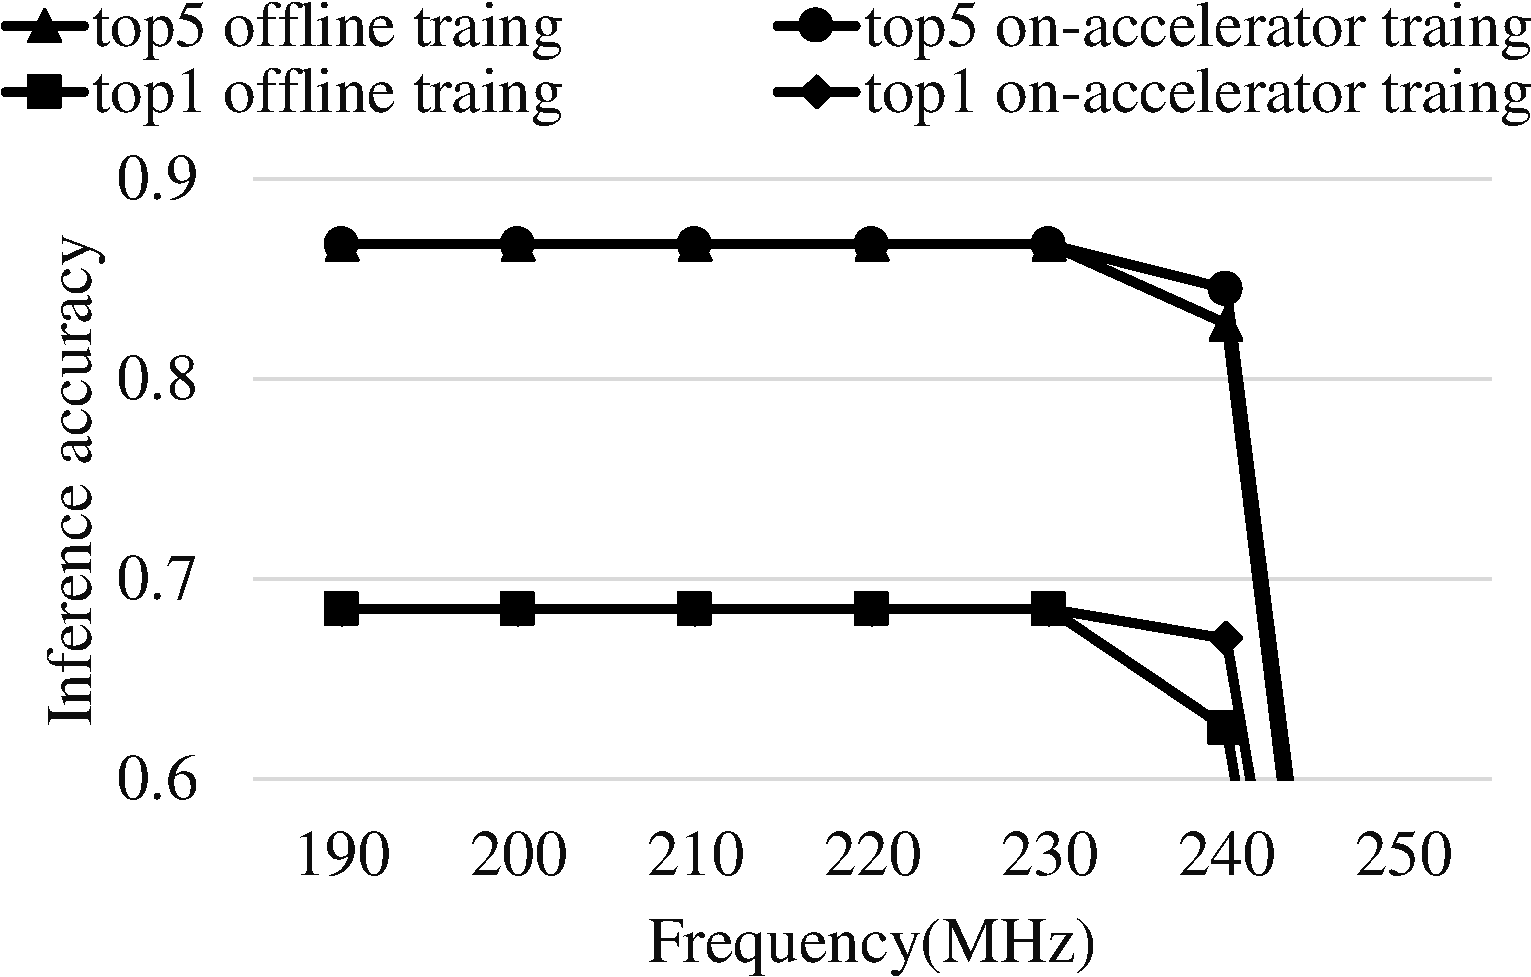
\includegraphics[width=0.65\linewidth]{accuracy_vgg16}
        }
        \qquad
	\subfloat[VGG-19]{
                \label{fig:vgg19_accuracy}
                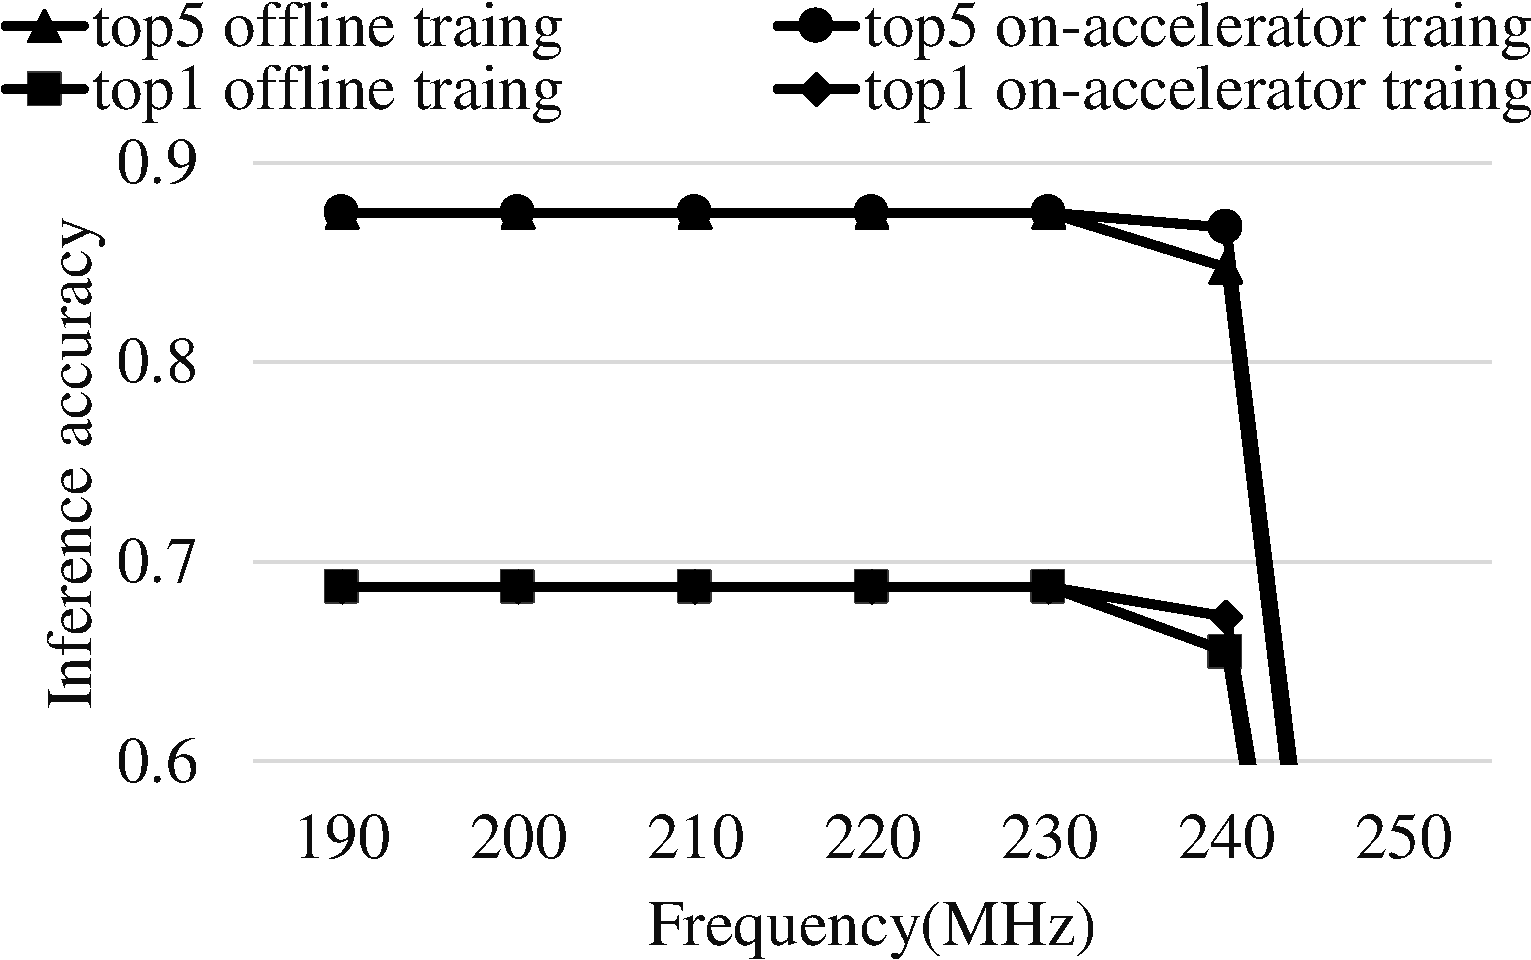
\includegraphics[width=0.65\linewidth]{accuracy_vgg19}
        }
	\caption{The prediction accuracy of the benchmark neural networks on accelerators with different overclocking}
        \label{fig:overclock-accuracy}
		\vspace{-1em}
\end{figure}

We further evaluate the normalized performance over the original CNN accelerators.
As given in Fig \ref{fig:relative_time_overclock}, the performance with the extreme accelerator 
overclocking achieves 1.25X speedup on average compared to the baseline design. 
We use EDP as the energy efficiency metric and compare the 
different overclocking configurations as exhibited in Fig \ref{fig:relative_energy_overclock}.
According to the figure, overclocking on FPGA based CNN 
accelerators achieves more significant energy efficiency improvement when 
compared to the performance improvement. A key reason is that 
the power consumption does not scale much with the clock frequency due to the 
relatively higher background power consumption. On the contrast, 
the performance which contributes more to the EDP metric scales 
much better. 

\begin{figure}
        \center{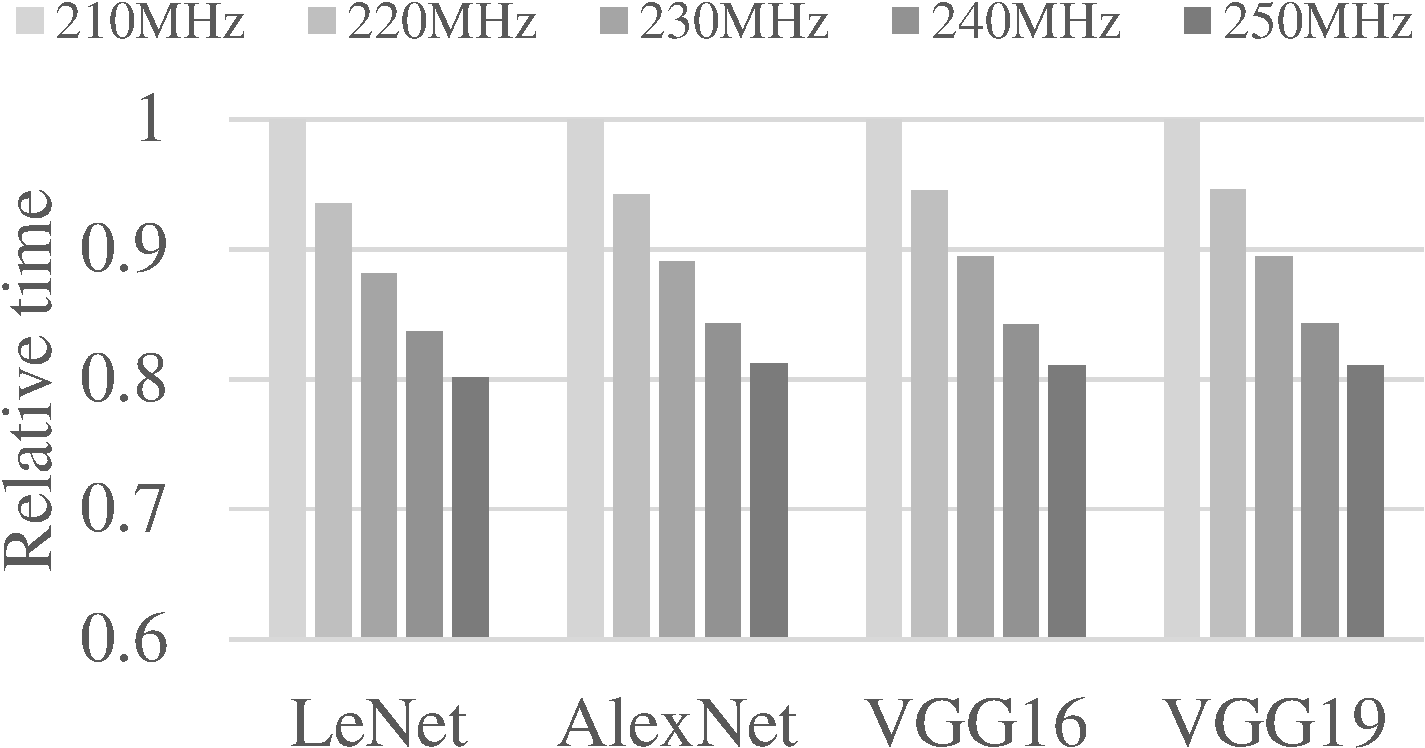
\includegraphics[width=0.65\linewidth]{relative_time_overclock}}
    \caption{Normalized performance of neural networks executed on CNN accelerators with different overclocking.}
\label{fig:relative_time_overclock}
\vspace{-1em}
\end{figure}

\begin{figure}
        \center{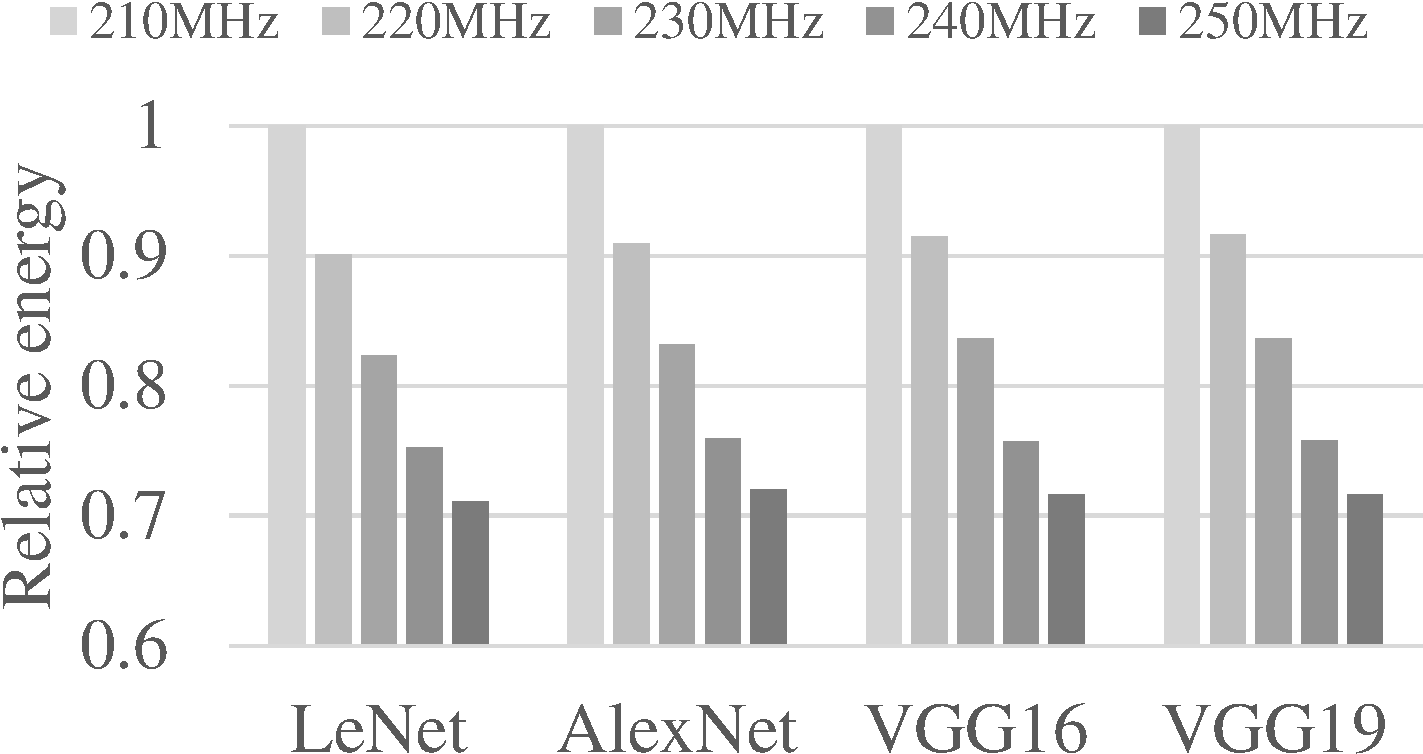
\includegraphics[width=0.65\linewidth]{relative_energy_overclock}}
    \caption{Normalized EDP of neural networks executed on CNN accelerators with different overclocking.}
\label{fig:relative_energy_overclock}
\vspace{-1em}
\end{figure}

In order to quantize the exact computing errors caused by overclocking, we 
particularly analyze the last layer output of the neural networks which 
is typically a vector. We compare it with the output without overclocking.
And we use the percentage of changed output data and the Euclidean distance 
of the output vectors to characterize the difference. 
The comparison is presented in Table \ref{tab:fr_ed}. It can be observed that 
computing errors can be completely hidden by the neural networks when the clock 
frequency is less than 240 MHz in the experiment. Moreover, the small Euclidean indicates that 
the computing error amplitude is relatively small though the percentage of 
the affected results is high when the clock is higher than 240 MHz.

\begin{table}
        \centering
        \vspace{-0.3em}
        \caption{Fault rate and Euclidean distance on the last output layer of the neural network}
        \label{tab:fr_ed}
        \vspace{-0.3em}
        \begin{tabular}{c|cccccc}
                \toprule
                Frequency(MHz) & 210 & 220 & 230 & 240 & 250 & 260 \\
                \midrule
                Euclidean distance & 0 & 0 & 0 & 0 & 35.2 & 104.8 \\
		\midrule
                Fault rate(\%) & 0 & 0 & 0 & 0 & 56.6 & 72.1 \\
                \bottomrule
        \end{tabular}
        \vspace{-1em}
\end{table}

\subsection{Optimization trade-offs}
As discussed in this paper, the timing error can be affected by many factors and it may change 
at runtime. There is no guarantee that the behavior of the CNN accelerator can keep stable even 
overclocking is just slightly higher than the original clock. We use the accelerator overclocked at the 
tipping point to perform the neural network computing. Then we keep measuring its 
prediction accuracy. As shown in Fig \ref{fig:stability}, we find that the accuracy is rather stable.
Although we still can not ensure the stability of the overclocked CNN accelerator, we can 
be sure that the probability of the severe errors such as accelerator hangup or considerable 
accuracy loss is rather low. As we did not observe the cases after processing 100000 pictures, 
we assume the probability of an severe error when processing an input picture is lower than 1/100000.

\begin{figure}
	\center{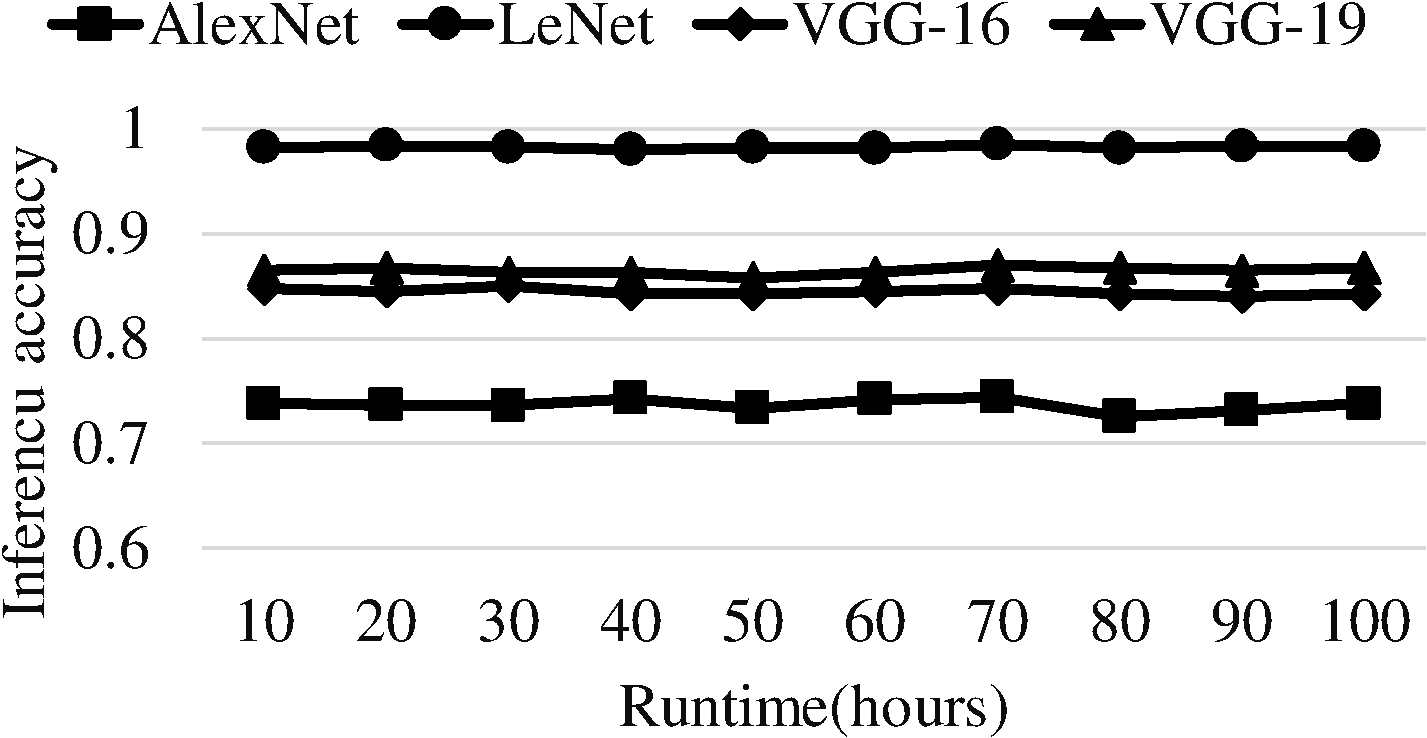
\includegraphics[width=0.65\linewidth]{stability}}
    \caption{Overclocking stability analysis}
\label{fig:stability}
\vspace{-1em}
\end{figure}

\begin{figure}
        \center{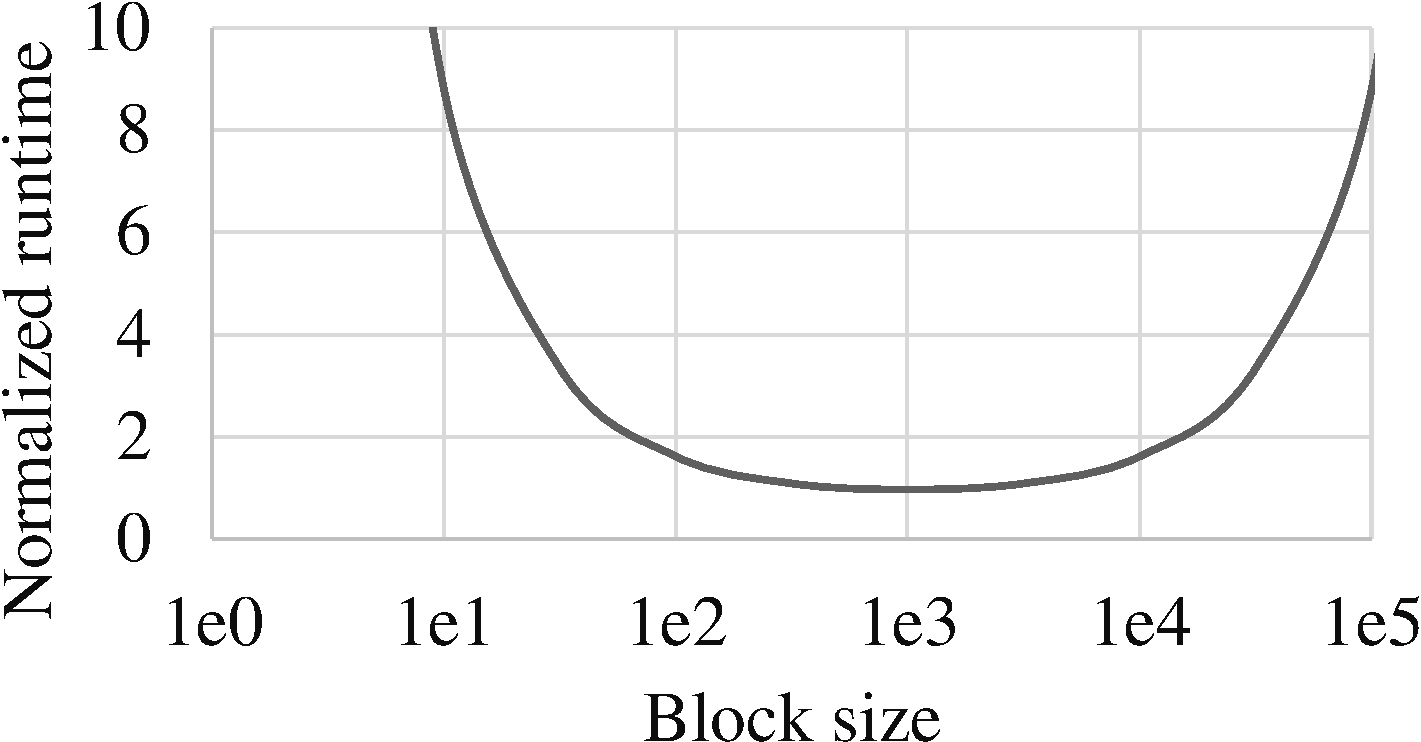
\includegraphics[width=0.65\linewidth]{cost_batch}}
    \caption{The relative overclocking runtime with different block size.}
\label{fig:cost_block}
\vspace{-1em}
\end{figure}

\begin{figure}
	\center{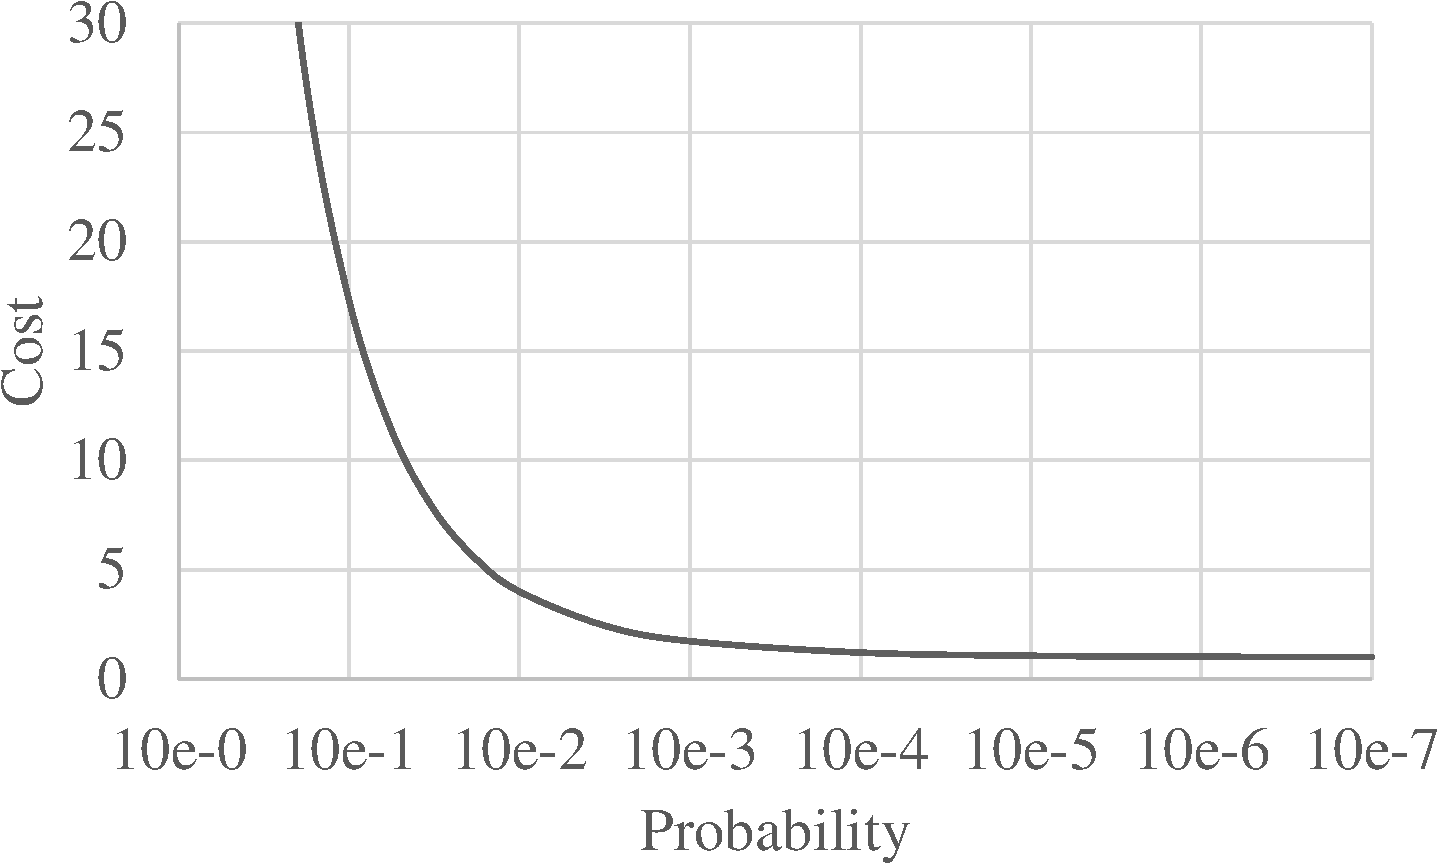
\includegraphics[width=0.65\linewidth]{cost_probability}}
    \caption{The relative overclocking runtime with different fault rate.}
\label{fig:cost_probability}
\vspace{-1em}
\end{figure}


With the severe errors, we need to invoke the checkpoint-based error recovery strategy. 
However, this strategy incurs cost including error detection and error recovery. 
We evaluate the overhead of the checkpoint-based strategy. 
A few parameters are critical to the overhead. One of them is the block size, which 
decides the granularity of checkpoint. One of them is the critical 
fault rate. It refers to the probability that CNN accelerator got severe errors 
when processing a single input figure. Another one is the reference data size.


Suppose reference data size is 100 and fault rate under 250 MHz is 1E-5. The relative runtime 
of overclocking over the normal design without overclocking is shown 
in Fig \ref{fig:cost_block}. When the block size is too big, the roll back cost will be 
too large and incurs additional runtime. When the block size is too small, the inserted 
reference data becomes non-trivial and the overall runtime also gets deteoriated. There is 
an optimal block size given specified fault rate and reference data size.
We also analyze the trend of the relative runtime under different fault rate.
As shown in Fig \ref{fig:cost_probability}, the relative runtime increases slightly at 
lower relative fault rate range but grows rapidly when the fault rate is larger than 1E-5.



\section{Conclusion} \label{sec:Conclusion}
In this work, we propose to replace the forward computing on GPPs with accelerator 
computing during training and have both the computing 
errors and the application data learned in the neural network models. 
In addition, we opt to protect critical neural layers to reduce the negative 
influence of computing errors.  
With the proposed resilient neural network training, 
the prediction accuracy of the retrained neural network models improves significantly 
when computing errors appear. 


%\appendix
%\section{Acknowledgement}

%\begin{acks}
%  The authors would like to thank Sam Ho for providing the suggestions on
%  HLS design debugging and optimization as well as the SDAccel usage. 

%\end{acks}


\bibliographystyle{IEEEtran}
\bibliography{refs} 


% trigger a \newpage just before the given reference
% number - used to balance the columns on the last page
% adjust value as needed - may need to be readjusted if
% the document is modified later
%\IEEEtriggeratref{8}
% The "triggered" command can be changed if desired:
%\IEEEtriggercmd{\enlargethispage{-5in}}

% references section

% can use a bibliography generated by BibTeX as a .bbl file
% BibTeX documentation can be easily obtained at:
% http://mirror.ctan.org/biblio/bibtex/contrib/doc/
% The IEEEtran BibTeX style support page is at:
% http://www.michaelshell.org/tex/ieeetran/bibtex/
%\bibliographystyle{IEEEtran}
% argument is your BibTeX string definitions and bibliography database(s)
%\bibliography{IEEEabrv,../bib/paper}
%
% <OR> manually copy in the resultant .bbl file
% set second argument of \begin to the number of references
% (used to reserve space for the reference number labels box)
%\begin{thebibliography}{1}

%\bibitem{IEEEhowto:kopka}
%H.~Kopka and P.~W. Daly, \emph{A Guide to \LaTeX}, 3rd~ed.\hskip 1em plus
%  0.5em minus 0.4em\relax Harlow, England: Addison-Wesley, 1999.

%\end{thebibliography}




% that's all folks
\end{document}


